\documentclass{article}
\usepackage[utf8]{inputenc}
\usepackage{multirow}
\usepackage{graphicx}
\usepackage{url}
\usepackage{tabularx}
\usepackage[titletoc]{appendix}
\begin{document}
\begin{titlepage}
\title{IOS-App}
\author{Johannes Franz und Normen Krug} 
	\title{Erweiterung der Stundenplan App um \newline Push Notifications}
	\date{Wintersemester 2017/2018} 
	\maketitle 
\end{titlepage}
\renewcommand{\contentsname}{Inhaltsverzeichnis}
\tableofcontents 
\newpage

\section{Einleitung}
Push Notifications sind ein fester Bestandteil vieler Apps. Deswegen soll die Stundenplan App um solche erweitert werden. Ziel soll es sein den Benutzer über Stundenplanänderungen aktiv zu informieren, um speziell auf kurzfristige Änderungen reagieren zu können. Ein Server überprüft dabei eine Stundenplan Datenbank auf Änderungen und sendet eine Push Notification an alle iOS Geräte, die sich für die jeweilige Vorlesung registriert haben. Ein Apache Webserver stellt dabei mit einer MySQL Datenbank und entsprechenden Chronjobs das Backend bereit.

Github: \url{https://github.com/HochschuleHofStundenplanapp}



\section{Projektfortschritt}
Um den Projektfortschritt nachvollziehen zu können, wurde dieser tabellarisch in Verbindung mit dem aktuellen Datum aufgelistet.\\


\noindent%
\begin{tabularx}{\textwidth}{|p{.25\textwidth}|X| }
\hline
\textbf{Datum} & \textbf{Erreichter Meilenstein}  \\ \hline 

Vorlesungsbeginn & Themenfindung \\ \hline

Siri & Einarbeitung in Siri. Erkennen erster Hürden. \\ \hline

Neue Themenfindung & Verwerfen von der Siri Projektidee und neue Themenfindung. \\ \hline

Festlegung & Thema Push Notifications festgelegt und Beginn der Einarbeitung. \\ \hline

28.10.2017 & Push Notifications lassen sich per PHP Script an einen fest eingestellten Token schicken \\ \hline

30.10.2017 & Eine Test iOS App kann per php Script mittels MAMP lokal eine Push Notification senden. \newline
Datenbank lokal in PhpMyAdmin angelegt. \newline
PHP Script schreibt bei Aufruf in die angelegte SQL Datenbank. \newline
Einarbeitung und Konvertierung der Dokumentation in Latex.
 \\ \hline
 31.10.2017 & Die Test iOS App wurde so erweitert, dass ein JSON File per POST Nachricht übermittelt werden kann.\newline
Das PHP Script parst nun das ankommende JSON File und fügt per insert die geparsten Daten in die Datenbank ein.\newline 
Einarbeitung in bestehende Schnittstelle und Überlegungen wie das bestehende Backend erweitert werden muss. 
 \\ \hline
 
 

\end{tabularx}

\newpage
\section{Umsetzung}

Apple bietet für die Umsetzung von Push Nachrichten den Apple Push Notification service (APNs) an. Dabei handelt es sich um einen bei Apple gehosteten Dienst, der Push Notifications per API ermöglicht.


\section{Aufgetretene Probleme}
- Zertifikate sehr verwirrend
- Bundle identifier und App Capabilities nach einem Git pull
- Komplexes Testen (Lokale Server, unterschiedliche Datei- und Serverstände) 
- Kein Zugriff auf die Git Schnittstelle.



\newpage
\section{Anhang}
\begin{figure}[h]
%	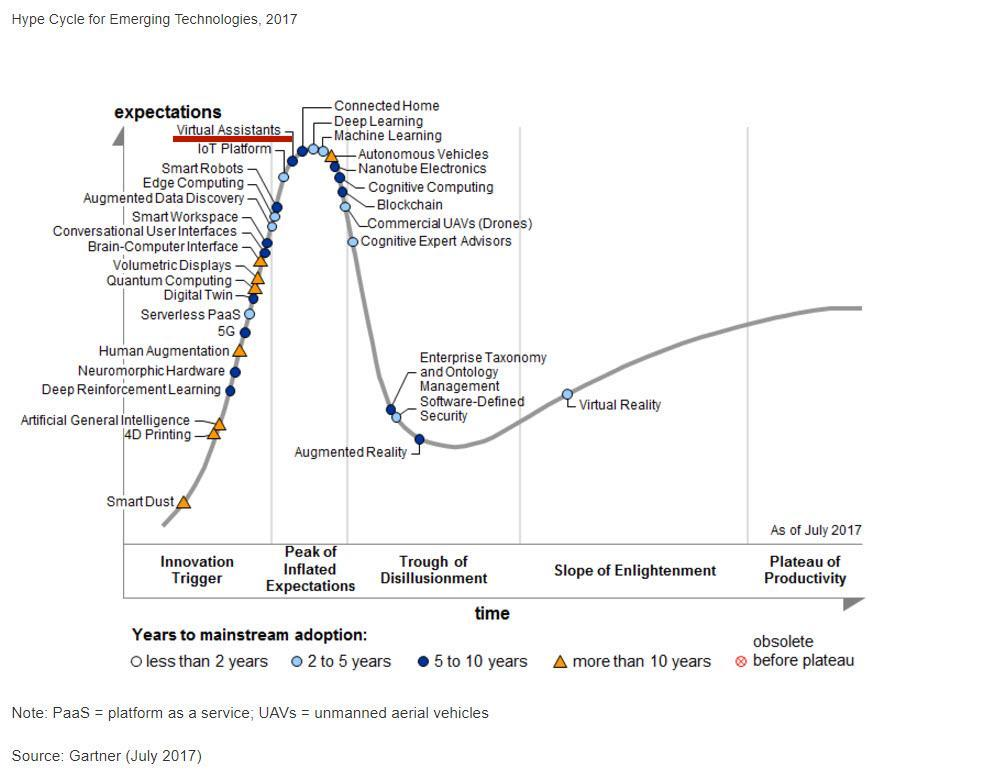
\includegraphics[width=15cm]{hype-cycle-for-emerging-technologies-2017}
\end{figure}

\newpage
\section{Eigenständigkeitserklärung}

\end{document}

